\documentclass[12pt]{article}
\usepackage{indentfirst}
\usepackage[utf8x]{inputenc}
\usepackage[T1]{fontenc}
\usepackage[english,lithuanian]{babel}
\usepackage{array}
\usepackage{caption}
\usepackage{makecell}
\usepackage[euler]{textgreek}
\usepackage{hyperref}
\usepackage{multirow}
\usepackage{boldline}
\usepackage{floatrow}
\floatsetup[table]{capposition=top}
\usepackage{amsmath, amsthm, amssymb}
\usepackage{graphicx}
\usepackage{setspace}
\usepackage{verbatim}
\usepackage[left=3cm,top=2cm,right=1.5cm,bottom=2cm]{geometry}
\usepackage{floatrow}
\newfloatcommand{capbtabbox}{table}[][\FBwidth]
\usepackage{blindtext}
\onehalfspacing

\newcommand{\EE}{\mathbb{E}\,} % Mean
\newcommand{\ee}{{\mathrm e}}  % nice exponent
\newcommand{\dd}{{\mathrm d}}
\newcommand{\RR}{\mathbb{R}}

\begin{document}
\selectlanguage{lithuanian}

\begin{titlepage}
\vskip 20pt
\begin{center}

\includegraphics[scale=0.5]{MIF}
\end{center}

%%%%%%%%%%%%%%%%%%%%%%%%%%%%%%%
% TITULINIO PUSLAPIO TEKSTAS
%%%%%%%%%%%%%%%%%%%%%%%%%%%%%%%

\vskip 20pt
\centerline{\bf \large \textbf{VILNIAUS UNIVERSITETAS}}
\bigskip
\centerline{\large \textbf{MATEMATIKOS IR INFORMATIKOS FAKULTETAS}}
\bigskip
\centerline{\large \textbf{BIOINFORMATIKOS BAKALAURO STUDIJŲ PROGRAMA}}

\vskip 90pt
\begin{center}
    {\bf \LARGE Tbx5 transkripcijos faktoriaus tyrimas \emph{Mus musculus}
     širdies ląstelėse}
\end{center}
\begin{center}
    {\bf \Large Research of Tbx5 transcription factor in \emph{Mus musculus}
     heart cells}
\end{center}
\vskip 20pt
\centerline{\bf \large \textbf{Kursinis darbas}}
\bigskip
\vskip 40pt

\hskip 140pt {\large Autorius: Danielė Stasiūnaitė}

\hskip 140pt{\large VU el. p.: (daniele.stasiunaite@mif.stud.vu.lt)}
\bigskip
\vskip 20pt

\hskip 140pt {\large Darbo vadovas: J. m. d. Kotryna Kvederavičiūtė}
\vskip 60pt
\vskip 40pt
\centerline{\large \textbf{Vilnius}}
\centerline{\large \textbf{2022}}
\newpage
\end{titlepage}

\selectlanguage{lithuanian}

%%%%%%%%%%%%%%%%%%%%%
% TURINIO PUSLAPIS
%%%%%%%%%%%%%%%%%%%%% 
\tableofcontents
\newpage

%%%%%%%%%%%%%%%%%%%%%%%%%%%%%%%%%%%%
% LIETUVIŠKOS SANTRAUKOS PUSLAPIS
%%%%%%%%%%%%%%%%%%%%%%%%%%%%%%%%%%%%

\section*{Santrauka}
Širdies regeneracijos procesų tyrinėjimas yra svarbi sritis, galinti
prisidėti prie širdies ligų  gydymo bei širdies audinių atstatymo po
pažeidimų (pvz., širdies raumens plyšimo). Sėkmingam ląstelių regeneracijos
taikymui praktikoje svarbu suprasti šio proceso mechanizmus bei išsiaiškinti
juose dalyvaujančius genus bei jų svarbą.

Tbx5 - Tbx5 geno koduojamas vienas iš daugelio kardiogeninių transkripcijos
faktorių, aktyvuojančių genus, kurie dalyvauja širdies vystymosi
embriogenezės metu bei audinio atstatyme regeneracijos metu.
                                                                                     
Šiame darbe naudojantis R programavimo kalbos bibliotekomis bei
bioinformatiniais komandinės eilutės bei internetiniais duomenų apdorojimo
bei analizės įrankiais išanalizuota, kokiuose ChIP sekoskaitos metodu gautų
naminės pelės (lot. \emph{Mus musculus}) ląstelių pikų mėginiuose Tbx5
transkripcijos faktoriaus motyvų yra daugiausiai bei kokie motyvai gali būti
identifikuoti analizuojamuose mėginiuose.

<TAISYTI>

Atlikta analizė parodė, kad 
Atliktos analizės metu mėginiuose identifikuota daug skirtingų motyvų,
susijusių su audinių regeneracijos metu vykstančiais procesais.
Daugiausiai tyrinėjamo Tbx5 transkripcijos faktoriaus motyvų identifikuota
naminių pelių embrionų fibroblastų ląstelėse, kurioms papildomai veiktos
kitais kardiogeniniais transkripcijos faktoriais. Rezultat. Mažiausias Tbx5 transkripcijos faktoriaus motyvų skaičius
būdingas fibroblastams, kurie buvo veikti ne pilnu kardiogeninių faktorių
rinkiniu.

<TAISYTI>

\hfill \break
\textbf{Raktiniai žodžiai:} ChIP sekoskaita, transkripcijos faktorius, Tbx5,
        pikas, motyvas, R.
\newpage

%%%%%%%%%%%%%%%%%%%%%%%%%%%%%%%%%%%%%%%%
% ANGLIŠKOS SANTRAUKOS PUSLAPIS
%%%%%%%%%%%%%%%%%%%%%%%%%%%%%%%%%%%%%%%%
<TAISYTI>
\section*{Summary}
The investigation of regeneration processes is an important field of research
that plays a significant role in the treatment of various diseases and injuries.
Therefore, it is mandatory to determine and apprehend the mechanisms and gene
products that regulate regeneration processes.

In this work, the analysis of the ChIP sequencing peaks samples that were
retrieved from different house mouse (lat. \emph{Mus musculus}) cells was
conducted using functions from R programming language libraries and performing
analysis steps using bioinformatics command-line tools and online services
in order to determine what type of house mouse cells has the greatest number
of Tbx5 transcription factor motifs and what factors might have an impact on
total Tbx5 motif hit count differences among house mouse genome sequences.

The undertaken analysis identified an ample number of motifs. An abundance
of key interest Tbx5 transcription factor was identified in the second
chromosome of house mouse embryonic fibroblasts that were treated with
serine/threonine kinase 1 (Akt1) and GATA4, HAND2, MEF2C cardiogenic
transcription factors. The least count of Tbx5 transcription factor motifs
is common for fibroblasts that were not treated with complete cardiogenic
transcription factor set. 
<TAISYTI>
\hfill \break
\textbf{Keywords:} ChIP-seq, transcription factor, Tbx5, peak, motif, R.
\newpage

%%%%%%%%%%%%%%%%%%%
% ĮVADO PUSLAPIS
%%%%%%%%%%%%%%%%%%%

\section{Įvadas}
\subsection*{Darbo temos aktualumas}

Spartėjanti mokslo raida, įvairūs atradimai bei išradimai stipriai paspartino
ir pagerino įvairių ligų diagnostikos bei prevencijos tyrimus, praplėtė žinias
ląstelės biologijos, genetikos, fiziologijos ir kitose srityse. Viena iš
medicinos sričių, kuri pradėta tyrinėti dar XVIII a., kai buvo nustatyta, kad
kai kurie organizmai geba atsiauginti prarastas arba sužeistas galūnes bei
kitus kūno audinius\cite{REGENERATION}, yra organizmų audinių bei organų
regeneracija.

Šiais laikais regeneracijos tyrimai atliekami su hidromis, planarijomis,
tritonais bei zebražuvėmis\cite{ORGANISMS}, siekiant išsiaiškinti šių organizmų
audinių regeneracijos mechanizmus bei pritaikyti žmonėms, patyrusiems traumas
ar turintiems specifinių kūno audinių pažeidimų. Regeneracijos procese
pagrindinę funkciją atlieka kamieninės ląstelės bei įvairūs transkripcijos
reguliavimo faktoriai, gebantys prisijungti prie DNR chromatino ir skatinti
arba slopinti specifinių genų transkripciją.

Sėkmingam regeneracijos procesų mechanizmų supratimui būtina išsiaiškinti, 
kokie transkripcijos faktoriai dalyvauja šiame procese bei kokias funkcijas jie
atlieka.

\subsection*{Darbo tikslas}

Patikrinti, ar skirtingų poveikių taikymas \emph{Mus musculus} širdies
ląstelėms daro didelę įtaką Tbx5 transkripcijos faktoriaus motyvų skaičiui.

\subsection*{Uždaviniai}
\begin{itemize}
    \item Išanalizuoti straipsnius bei pasirinkti tinkamiausius tyrimo duomenis.
    \item Įvertinti pikų skirtumus tarp mėginių, taikant skirtingus statistinių
        duomenų vaizdavimo būdus.
    \item Nustatyti, kokioms širdies ląstelėms būdingas didžiausias Tbx5
        transkripcijos faktoriaus motyvo atitikimų skaičius.
    \item Atlikus de novo motyvų paiešką, nustatyti, kokios biologinės
        funkcijos yra būdingos identifikuotiems motyvams.
\end{itemize}

\newpage

%%%%%%%%%%%%%%%%%%%%%
% DUOMENŲ APŽVALGA
%%%%%%%%%%%%%%%%%%%%%

\section{Duomenų bazės ir duomenys}
\subsection{GTRD duomenų bazė}
Tyrimui naudoti duomenys atsisiųsti iš GTRD (Gene Transcription Regulation
Database)\cite{GTRD} duomenų bazės, saugančios informaciją apie transkripcijos
sekų ir atviro chromatino regionus. Taip pat duomenų bazėje saugomi
nekartografuojamų regionų duomenys bei potencialūs žmonių bei naminių pelių
regionai, prie kurių gali jungtis transkripcijos faktoriai.

Ši duomenų bazė pasirinkta dėl sistemiškai surinktų ChIP-seq eksperimentų,
kurių metu gauti rezultatai yra unifikuotai apdoroti ir paruošti tyrėjų
meta-analizėms.

GTRD duomenų bazėje duomenys saugomi binariniu anotacijų formatu \emph{bigBed},
leidžiančiu atvaizduoti pasirinktą chromosomos regioną interaktyviose genominės
informacijos vizualizavimo naršyklėse (pavyzdžiui, UCSC Genome
Browser\cite{UCSCGB}) efektyviau nei tekstinis BED formatas.

\subsection{Pasirinktų mėginių charakteristika}
Analizė atlikta, naudojantis 3 nepriklausomais eksperimentais, kuriuos iš viso
sudarė 7 skirtingi mėginiai. Pirmoje lentelėje (1 lentelė) pateikta informacija
apie tyrimui atlikti naudotus duomenis, surinktus iš naminės pelės
(lot. \emph{Mus musculus}) ląstelių.

\begin{table}[htb]
    \newcolumntype{M}[1]{>{\centering\arraybackslash}m{#1}}
    \small
    \caption*{\small\textbf{1 lentelė. Mėginių charakteristikos}}
    \begin{tabular}{|c|c|c|c|c|c|c|}
    \hline
    %\thead{Sample\\ window}
    \textbf{GTRD ID} & \textbf{Ląstelių tipas} &
        \textbf{\thead{Kamienas}} & \textbf{\thead{Poveikis}} &
        \textbf{Antikūnai} & \textbf{PubMed ID}\\
    \hline
    EXP030898 & \thead{HL - 1\\ (širdies raumens)} & C57BL/6J &
                \thead{TRE\\ promotorius (2 d.)} & - & 21415370\cite{ARTCL1}\\ 
    \hline
    EXP058852 & Širdies prieširdžių & C57BL/6 & - &
                \thead{Tbx5\\ (sc-17866)} & 31080136\cite{ARTCL2}\\
    \hline
    EXP062056 & \thead{Pelių naujagimių širdies\\ fibroblastų, 
                ekspresuojančių\\ didelį kiekį T antigeno, linija} & CD1 &
                \thead{sb431542,\\ xav939} & \thead{anti-TBX5\\ (sc-17866x)} &
                31271750\cite{ARTCL3}\\
    \hline
    EXP058843 & \thead{MEF\\ (embrionų fibroblastai)} & C57BL/6 &
                AGHMT (2 d.) & \thead{anti-Tbx5\\ (sc-17866)} &
                31080136\cite{ARTCL2}\\
    \hline
    EXP058847 & \thead{MEF\\ (embrionų fibroblastai)} & C57BL/6 & GHMT (2 d.) &
                \thead{Tbx5\\ (sc-17866)} & 31080136\cite{ARTCL2}\\
    \hline
    EXP058850 & \thead{MEF\\ (embrionų fibroblastai)} & C57BL/6 & GMT (2 d.) &
                \thead{Tbx5\\ (sc-17866)} & 31080136\cite{ARTCL2}\\
    \hline
    EXP058856 & \thead{MEF\\ (embrionų fibroblastai)} & C57BL/6 &
                \thead{vienas\\ faktorius (2 d.)} & \thead{Tbx5\\ (sc-17866)} &
                31080136\cite{ARTCL2}\\
    \hline
    \end{tabular}
\end{table}

\newpage

\subsection{Santrumpų bei pavadinimų paaiškinimai}
\begin{itemize}
    \item \textbf{HL - 1}: pelių širdies raumens ląstelės, išgautos iš
        navikinių prieširdžių kardiomiocitų linijos. Šios ląstelės gali
        betarpiškai dalintis ir spontaniškai keisti savo formą, vykstant
        širdies raumens susitraukimo/atsipalaidavimo procesams.
    \item \textbf{MEF}: pelių embrionų fibroblastai (angl. \emph{Mouse
        Embryonic Fibroblast}). Šiai ląstelių linijai būdingas ląstelių
        gyvybingumo apribojimas, reiškiantis, jog šios ląstelės greitai
        pasensta ir miršta.
    \item \textbf{C57BL/6}: inbrydingo (angl. \emph{inbreeding}) būdu išvestų
        naminių pelių veislė. Šios veislės pelėms būdingas itin tamsus
        kailis, padidėjęs jautrumas garsams, kvapams, skausmui ir žemai
        temperatūrai. Ši veislė dažnai naudojama nutukimą ir imuninę sistemą
        tiriančiuose tyrimuose.
    \item \textbf{C57BL/6J}: prie naminių pelių veislės pavadinimo pridėtos
        raidės patikslina, kurioje laboratorijoje veislės išvestos. 'J' raidė
        nurodo, kad pelių veislė išvesta Meino valstijoje (JAV) įsikūrusioje
        Džeksono laboratorijoje\cite{JCKSLAB}.
    \item \textbf{CD1}: autbrydingo (angl. \emph{outbreeding}) būdu išvestų
        naminių pelių veislė. Šios veislės pelėms būdingas baltas kailis.
        Taip pat CD1 pelės dažnai naudojamos genetiniuose, toksikologiniuose,
        farmakologiniuose ir senėjimo tyrimuose.
    \item \textbf{TRE}: tetraciklino atsako elementas (angl. \emph{Tetracycline
        Response Element}). Tai yra 7 DNR sekos fragmentai,
        sudaryti iš 19 nukleotidų ir atskirti trumpesniais sekų fragmentais.
    \item \textbf{sb431542}: stipriai veikianti, selektyvi cheminė medžiaga;
        transformuojančio augimo faktoriaus {\textbeta} (TGF-{\textbeta})
        inhibitorius.
    \item \textbf{xav939}: stipriai veikianti cheminė medžiaga; tankirazės
        inhibitorius. Tankirazė slopina TERF1 baltymo, stabdančio
        telomerazės veiklą, jungimąsi prie telomerinių DNR sekų.
    \item \textbf{AGHMT}: AKT1 - serino/treonino kinazė 1; GATA4, HAND2, MEF2C,
        Tbx5 - kardiogeniniai transkripcijos faktoriai.
    \item \textbf{GHMT}: GATA4, HAND2, MEF2C, TBX5 transkripcijos faktorių
        komplektas.
    \item \textbf{GMT}: GATA4, MEF2C, Tbx5 transkripcijos faktorių komplektas.
    \item \textbf{sc-17866x/ sc-17866}: iš ožkų išskirti antikūnai,
        atpažįstantys žmonių, pelių ir žiurkių Tbx5 antigeną.
\end{itemize}

\subsection{Pasirinktų eksperimentų apžvalga}
\begin{itemize}
    \item \textbf{EXP030898}: vienas mėginys iš septyniolikos eksperimento
        metu tirtų mėginių. Eksperimente buvo siekiama patvirtinti arba
        atmesti hipotezę apie širdies stipriklių (angl. \emph{enhancer})
        identifikiavimą prie chromatino jungiantis keliems transkripcijos
        faktoriams.

        HL - 1 širdies raumens ląstelės buvo infekuotos su adenovirusu,
        ekspresuojančiu troponiną T, kuris skatina \emph{rtTA} ir \emph{BirA}
        genų ekspresiją, bei TRE promotoriumi, skatinančiu Tbx5 transkripcijos
        faktoriaus geno raišką.
    \item \textbf{EXP058852}: prieširdžių ląstelės buvo du kartus po 24
        valandas laikytos mišinyje su retrovirusais. Papildomi poveikiai nebuvo
        taikyti.
    \item \textbf{EXP062056}: eksperimente ląstelės buvo infekuotos su GATA4,
        Mef2c, ir Tbx5 transkripcijos faktorius sintetinančiais retrovirusais.
        Ląstelės augintos terpėje, kurioje buvo {Tgf\textbeta} inhibitoriaus
        sb431542, skatinančio kardiomiocitų diferenciaciją iš pliuripotentinių
        kamieninių ląstelių, ir Wnt inhibitoriaus xav939, stabdančio
        nediferencijuotų ląstelių sintezę ir skatinančio progenitorinių
        ląstelių kardiomiogenezę.
\end{itemize}

Pasirinktų duomenų rinkinyje naudoti vieno eksperimento, kuriame buvo tirti
širdies ląstelių atsinaujinimo ir diferenciacijos mechanizmai, keturiais
skirtingais poveikiais tirti embrionų fibroblastų mėginiai:

\begin{itemize}
    \item \textbf{EXP058843}: embrionų fibroblastai veikti AGHMT. Esant
        prisijungusiems kardiogeniniams transkripcijos faktoriams, AKT1
        skatina fibroblastų diferenciaciją į širdies ląsteles - kardiomiocitus.
    \item \textbf{EXP058847}: neįtraukta AKT1 serino/treonino kinazė 1.
    \item \textbf{EXP058850}: į kardiogeninių transkripcijos faktorių mišinį
        neįtrauktas HAND2 transkripcijos faktorius.
    \item \textbf{EXP058856}: ląstelės veiktos tik vienu faktoriumi, kuris
        straipsnyje nebuvo specifikuotas.??????
  \end{itemize}
\newpage

%%%%%%%%%%%%
% METODAI
%%%%%%%%%%%%

\section{Tyrimo metodai}
Tbx5 transkripcijos faktoriaus pikų tyrimo analizė atlikta su R programavimo
kalba\cite{R} (4.2.0 versija).

Tarpiniams analizės rezultatams pateikti naudotas komandinės eilutės įrankis
Scikick\cite{SCIK} (0.2.0 versija), leidžiantis generuoti R Markdown (Rmd)
ataskaitas HTML formatu bei kurti struktūrizuotus puslapius, apjungiant
iš daugelio Rmd failų gautus HTML ataskaitų failus.

\subsection{Pikų skaičiaus nustatymas mėginiuose}
\emph{Tbx5} pikų skaičius skirtinguose mėginiuose apskaičiuotas su
standartine R ilgio funkcija \emph{length()}, kuri pritaikyta \emph{GRanges}
objektui, aprašančiam genomines pozicijas bei su jomis susijusias anotacijas.
Objektas sukurtas su \emph{rtracklayer}\cite{R_TRACK} bibliotekos funkcija
\emph{import()}.

Pikų skaičių mėginiuose atvaizduojanti stulpelinė diagrama sukurta su
\emph{ggplot2}\cite{R_GGPLOT} bibliotekos \emph{geom\_bar()} funkcija.

\subsection{Pikų skaičiaus nustatymas chromosomose}
Transkripcijos faktoriaus pikų skaičius skirtingose chromosomose kiekvienam
mėginiui apskaičiuotas, naudojantis standartine R funkcija \emph{length()},
pritaikyta atskiroms chromosomoms, kurių pozicijos aprašytos \emph{GRanges}
objekte. Gauti rezultatai normalizuoti apskaičiuotą pikų skaičių padalinus
iš kiekvienos chromosomos ilgio. Normalizavimas taikytas, siekiant įvertinti
pikų skaičių tarp chromosomų, nepriklausomai nuo chromosomos ilgio.

Kiekvieno mėginio Tbx5 transkripcijos faktoriaus pasiskirstymas
chromosomose atvaizduotas su \emph{ggplot()} ir papildoma funkcija
\emph{facet\_wrap()}, sukuriančia atskirus grafikus pagal pasirinktą elementą -
chromosomas.

\subsection{Persidengiančių pikų procentinė dalis}
Persidengiančių pikų tarp mėginių procentinė dalis nustatyta su modifikuota
\emph{Jaccard()} funkcija, apskaičiuojančia, kiek yra sutampančių regionų tarp
dviejų mėginių poros. Naudojantis nemodifikuota funkcija, Jaccard koeficientas
apskaičiuojamas pagal išraišką:

                \[ J(A, B) =  \frac{|A \cap B|}{|A \cup B|} \]

\emph{Jaccard} koeficientas gaunamas iš rinkiniams A ir B bendrų duomenų ilgio
padalinus dviejų duomenų rinkinių bendrą duomenų ilgį.

Modifikavus \emph{Jaccard} koeficiento gavimo funkciją, koeficientas
apskaičiuojamas pagal išraišką, kur sutampančių A ir B rinkinių duomenų ilgis
padalinamas iš A rinkinio ilgio:

                    \[ J(A, B) = \frac{|A \cap B|}{|A|} \]

\emph{Jaccard} koeficiento skaičiavimo funkcija modifikuota, nes skaičiuojant
koeficientą su standartine \emph{Jaccard} funkcija, gaunamas itin didelis
pikų sąjungos skaičius, o persidengiančių pikų skaičius gaunamas mažas,
todėl persidengiančių pikų skaičių padalinus iš pikų sąjungos gaunamas
itin mažas koeficientas, kurio apskaičiuota procentinė dalis neretai neviršijo
1\%.

Tam, jog būtų galima patikimiau įvertinti, kokia pirmojo mėginio procentinė
pikų dalis persidengia su antruoju mėginiu, persidengiančių pikų skaičius
padalintas iš pirmojo mėginio pikų skaičiaus.

Gauti rezultatai atvaizduoti spalvų intensyvumo grafike (angl. \emph{heatmap}),
sukurtame su \emph{ggplot()} ir papildoma funkcija \emph{geom\_tile()}.

\subsection{Tbx5 motyvo nustatymas}
Šiame etape genomines pozicijas aprašantys \emph{bigBed} formato failai
konvertuoti į BED formato failus, pasinaudojus UCSC komandinės eilutės programa
\emph{bigBedToBed}\cite{BBTOBED}.

Sugeneruoti BED formato failai panaudoti pikus atitinkančių sekų iš naminės
pelės genomo gavimui FASTA formatu. Sekos iš genomo išgautos, pasinaudojus
komandinės eilutės įrankio BEDTools\cite{BEDTOOLS} (2.30.0 versija) programa
\emph{getfasta}\cite{GET_FASTA}.

Kiekviename mėginyje esančio Tbx5 transkripcijos faktoriaus motyvo procentinė
dalis apskaičiuota susumavus \emph{Biostrings}\cite{BIOSTR} bibliotekos
funkcijos \emph{countPWM()} rezultatus. Funkcijai \emph{countPWM()} kaip
argumentas pateikta Tbx5 transkripcijos faktoriaus pozicinė svorių matrica bei
mėginio nukleotidų sekų rinkinys FASTA formatu. Gauta funkcijos reikšmė
padalinta iš bendro pikų skaičiaus.

Pozicinė svorių matrica atsisiųsta iš HOCOMOCO\cite{HOCOMOCO} (11.0 versija)
(angl. \emph{HOmo sapiens COmprehensive MOdel COllection}) duomenų bazės
\emph{Homo sapiens} ir \emph{Mus musculus} organizmų transkripcijos faktorių
kolekcijos. Pozicinę svorių matricą atitinkantis sekos logotipas vaizduojamas
pirmame paveiksle (1 pav.).

\begin{figure}[htb]
    \begin{center}
        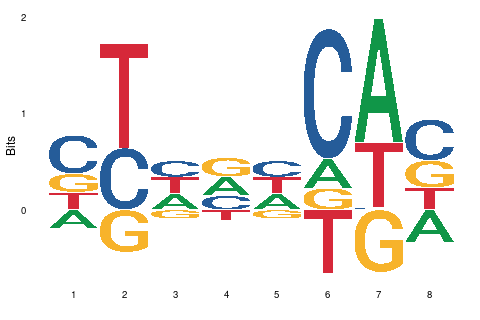
\includegraphics[width=0.5\linewidth]{../Figures/tbx5_motif.png}
        \vspace{-2\baselineskip}
        \caption*{\small\textbf{1 pav. Tbx5 transkripcijos faktoriaus
                                sekos logotipas}}
    \end{center}
\end{figure}

Identifikuotų Tbx5 transkripcijos faktoriaus motyvų skaičius vizualizuotas su
pagrindinėmis \emph{ggplot()} ir \emph{geom\_bar()} funkcijomis.

\subsection{Motyvų paieška \emph{de novo}}
Praturtintų sekų radimui panaudota komandinės eilutės įrankio HOMER\cite{HOMER}
(v4.11 versija) programa \emph{findMotifsGenome.pl}, analizuojanti BED formato
failus (faile specifikuotas pozicijas), ir ieškanti praturtintų sekų atitikimo
anotuotame naminės pelės \emph{mm10} referentiniame genome. Tarp mėginių
sutampantys motyvai nustatyti, naudojantis R biblioteka
\emph{UpSetR}\cite{UPSETR}.

\subsection{Praturtintų sekų biologinių funkcijų nustatymas}
Identifikuotų motyvų biologinės funkcijos nustatytos, pasinaudojus
UniProt\cite{UNIPROT} duomenų bazės genų ontologijos (angl. \emph{Gene
Ontology (GO)}) biologinių procesų, ląstelinių komponentų ir molekulinių
funkcijų klasifikacija.

\subsection{Analizės eigos schema}
Antrajame paveiksle (2 pav.) vaizduojama analizės etapus apibendrinanti schema:
\begin{figure}[htb]
    \begin{center}
        \includegraphics[width=1\linewidth]{../Figures/Diagrama.png}
        \vspace{-2\baselineskip}
        \caption*{\small\textbf{2 pav. Analizės atlikimo eiga}}
    \end{center}
\end{figure}

\newpage

%%%%%%%%%%%%%%%%%%%%%%%%%%%%%
% GAUTŲ REZULTATŲ APŽVALGA
%%%%%%%%%%%%%%%%%%%%%%%%%%%%%

%%%%%%%%%%%%%%%%%%%%%%%%%%%%%%%%
% REGIONŲ SKAIČIUS MĖGINIUOSE
%%%%%%%%%%%%%%%%%%%%%%%%%%%%%%%%

\section{Rezultatai ir jų aptarimas}
\subsection{Pikų skaičiaus skirtumai tarp mėginių}
Prieš pradedant Tbx5 motyvo paiešką, visiems mėginiams taikytas statistinis
duomenų vizualizavimas, siekiant įvertinti ChIP sekoskaitos duomenis bei
nustatyti, kaip skiriasi mėginiai, kuriuose tirtoms panašioms ląstelėms
taikyti skirtingi poveikiai.
Trečiame paveiksle (3 pav.) pateikiamoje stulpelinėje diagramoje vaizduojamas
pikų skaičiaus pasiskirstymas skirtinguose mėginiuose.

\begin{figure}[htb]
    \begin{center}
        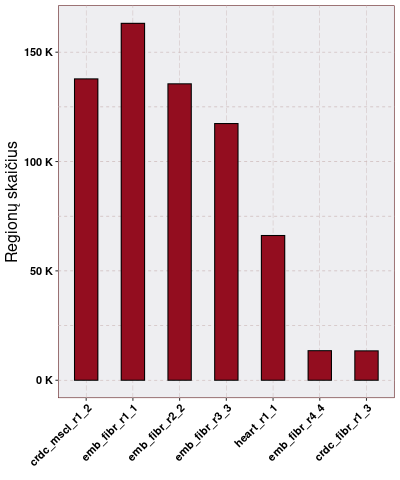
\includegraphics[width=0.5\linewidth]{../Figures/total_peak_counts.png}
        \vspace{-2\baselineskip}
        \caption*{\small\textbf{3 pav. Pikų skaičių mėginiuose vaizduojanti
                                stulpelinė diagrama}}
    \end{center}
\end{figure}

Remiantis diagrama didžiausias Tbx5 transkripcijos faktoriaus pikų skaičius
nustatytas mėginyje \small\emph{emb\_fibr\_r1\_1}, kuriame pelių embrionų
fibroblastų ląstelės veiktos AGHMT faktoriais.
Šį rezultatą palyginus su kitais to paties eksperimento mėginiais, kuriuose
tirtas tas pats pelių embrionų fibroblastų ląstelių kamienas, tačiau ląstelės
veiktos tik kai kuriais faktoriais, pastebimas gradualus Tbx5 transkripcijos
faktoriaus pikų skaičiaus mažėjimas diagramoje
\small\emph{emb\_fibr\_r2\_2}, \small\emph{emb\_fibr\_r3\_3} ir
\small\emph{emb\_fibr\_r4\_4} pavaizduotuose stulpeliuose (pažymėta
oranžine spalva). Tarp šių mėginių pikų skirtumai ypač ryškūs - pikų
skaičius skiriasi \(\sim\)25 tūkst. ir \(\sim\)100 tūkst. pikų.

Mažiausiai pikų nustatyta mėginyje, kuriame tirti pelių naujagimių širdies
fibroblastai paveikti inhibitoriais. Nepaisant to, kad abu inhibitoriai
skatina širdies ląstelių diferenciaciją\cite{HEART_CELL_DIFF_ARTCL} ir darant
prielaidą, kad ChIP sekoskaitos duomenys yra tikslūs ir juose nėra
metodo klaidų, mažas pikų skaičius rodo, kad papildomas veikimas inhibitoriais
gali daryti mažą įtaką transkripcijos faktoriaus jungimuisi prie DNR sekų.

Remiantis gautais rezultatais pikų skaičius skirtingais poveikiais veiktose
panašiose ląstelėse varijuoja itin stipriai, tačiau šiuos rezultatus reikia
vertinti atsargiai, atsižvelgiant į ChIP metodu gautų duomenų paruošimo
tikslumą ir teisingumą.

%%%%%%%%%%%%%%%%%%%%%%%%%%%%%%%%%%%%%%%%%%%%%
% PIKŲ SKAIČIUS ATSKIROSE CHROMOSOMOSE
%%%%%%%%%%%%%%%%%%%%%%%%%%%%%%%%%%%%%%%%%%%%%
<TAISYTI ATLIKUS NORMALIZAVIMĄ>
\subsection{Pikų pasiskirstymas chromosomose}
Antrajame statistinių duomenų vaizdavimo etape patikrinta, kaip mėginių pikai
pasiskirstę atskirose chromosomose, atlikus normalizavimą pagal chromosomų ilgį.

Vaizduojamuose grafikuose (4 pav.) didžiausias pikų skaičius nustatytas
pirmoje, antroje ir penktoje chromosomose. Naminės pelės pirmoji chromosoma yra
pati didžiausia, turinti 195 milijonų bazių porų, antroji chromosoma sudaryta
iš 182 megabazių, penktoji chromosoma - 152 milijonų bazių porų, todėl didesnis
regionų skaičius šiose chromosomose nėra neįprastas reiškinys. Kitose
chromosomose regionų skaičius yra mažesnis. Ypač mažas regionų skaičius
nustatytas devynioliktoje (61 Mbp), X (169 Mbp) ir Y (91 Mbp) chromosomose.

\begin{figure}[htb]
    \begin{center}
        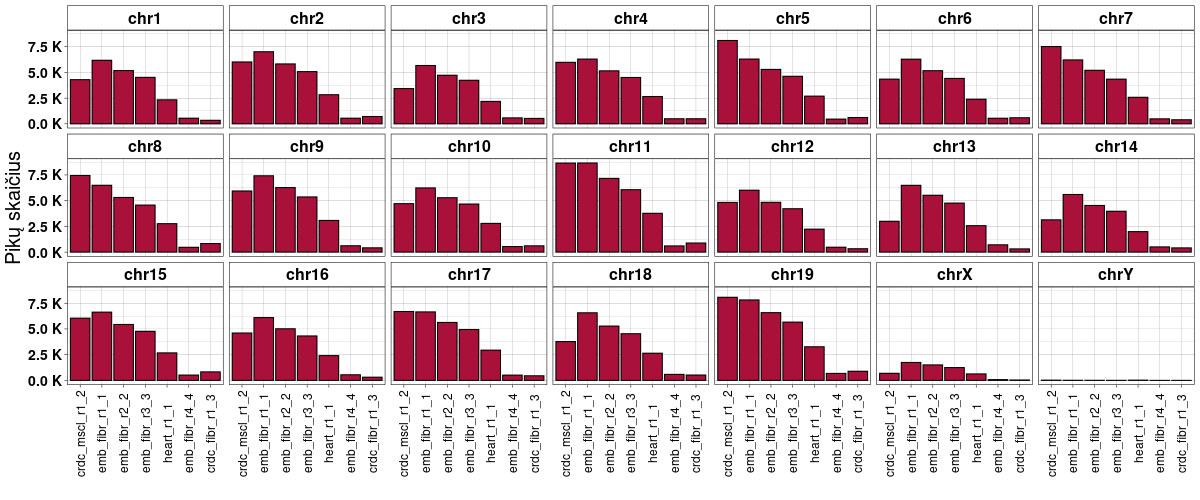
\includegraphics[width=1\linewidth]{../Figures/peak_counts_by_chr.png}
        \vspace{-2\baselineskip}
        \caption*{\small\textbf{4 pav. Pikų pasiskirstymas chromosomose}}
    \end{center}
\end{figure}

Biologinių replikų mėginiuose didžiausias regionų skaičius nustatytas antroje
chromosomoje. Taip pat grafikuose išsiskiria kontrolinis HL - 1 širdies
ląstelių mėginys, kuriame didžiausias regionų skaičius nustatytas penktojoje
chromosomoje.

<TAISYTI ATLIKUS NORMALIZAVIMĄ>

Remiantis pavaizduotomis regionų skaičiaus pasiskirstymo chromosomose
stulpelinėmis diagramomis, itin išsiskiriantis atrankumas chromosomų atžvilgiu
nenustatytas, todėl galima teigti, jog šiame analizės etape duomenų
problematiškumas nepastebimas arba jo nėra.

\newpage

%%%%%%%%%%%%%%%%%%%%%%%%%%%%%%%%%%%%%%%%%%%
% TARP MĖGINIŲ PERSIDENGIANTYS REGIONAI
%%%%%%%%%%%%%%%%%%%%%%%%%%%%%%%%%%%%%%%%%%%

\subsection{Tarp mėginių persidengiantys pikai}
Paskutiniame statistinių duomenų vaizdavimo etape nustatyta persidengiančių
mėginių duomenų procentinė dalis, siekiant įvertinti analizuojamų mėginių
panašumą.

\begin{figure}[htb]
    \begin{center}
        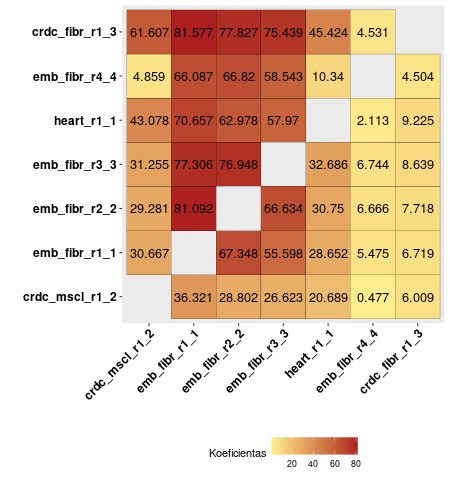
\includegraphics[width=0.6\linewidth]{../Figures/peak_overlaps.png}
        \vspace{-2\baselineskip}
        \caption*{\small\textbf{5 pav. Persidengiančių pikų procentinės
                                dalies spalvų intensyvumo grafikas}}
    \end{center}
\end{figure}

Remiantis pavaizduoto spalvų intensyvumo grafiko (5 pav.) duomenimis, didžiausi
persidengiančių pikų procentai nustatyti tarp šių mėginių:

\begin{itemize}
    \item \textbf{81.577 \%} - tarp mėginio, kuriame buvo tiriamos širdies
        fibroblastų ląstelės, veiktos inhibitoriais, ir mėginio, kuriame
        tirti embrionų fibroblastai, veikiant AGHMT.
    \item \textbf{81.092 \%} - tarp mėginio, kuriame tirti embrionų
        fibroblastai ir mėginio, kuriame nebuvo AKT1.
    \item \textbf{77.827 \%} - tarp mėginio su inhibitoriais veiktomis
        širdies fibroblastų ląstelėmis ir mėginio, kuriame nebuvo AKT1.
    \item \textbf{76.948 \%} - tarp mėginio, kuriame nebuvo HAND2 faktoriaus,
        ir mėginio, kuriame nebuvo AKT1.
    \item \textbf{75.439 \%} - tarp mėginio su inhibitoriais veiktomis
        širdies fibroblastų ląstelėmis ir tarp mėginio, kuriame nebuvo HAND2
        faktoriaus.
  \end{itemize}

\newpage

Remiantis spalvų intensyvumo grafiku didžiausius persidengiančių pikų skaičius
tarp mėginių turi tie patys mėginiai, kurie buvo nustatyti ir 4.1 bei 4.2
poskyriuose, todėl statistinis duomenų vaizdavimas, taikant vizualizavimo
funkcijas skirtingiems mėginių duomenims padeda įžvelgti duomenų skirtumus
ir grafikuose išskirti tuos pačius mėginius, turinčius maksimalias ir
minimalias reikšmes.

%%%%%%%%%%%%%%%%%%%%%%%%%%%
% TBX5 MOTYVO NUSTATYMAS
%%%%%%%%%%%%%%%%%%%%%%%%%%%

\subsection{Tbx5 motyvo pasiskirstymas mėginiuose}
Įvertinus vizualizuotų duomenų skirtumus, vykdomos analizės metu nustatyta,
kiek buvo nustatytas Tbx5 motyvo taikinių skaičius skirtinguose mėginiuose.
Rezultatas pateiktas šeštame paveiksle (6 pav.).

\begin{figure}[htb]
    \begin{center}
        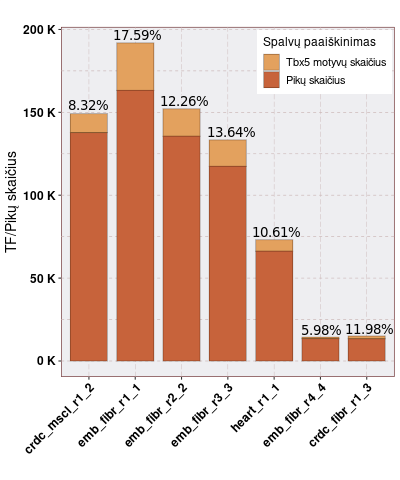
\includegraphics[width=0.5\linewidth]{../Figures/tf_hit_percentage.png}
        \vspace{-2\baselineskip}
        \caption*{\small\textbf{6 pav. Tbx5 motyvų atitikimų skaičiaus palyginimo
                                sudėtinė diagrama}}
    \end{center}
\end{figure}

Daugiausiai Tbx5 motyvo sekos taikinių nustatyta mėginyje,
kuriame embrionų fibroblastai veikti serino/treonino kinaze 1 (Akt1) bei
keliais transkripcijos faktoriais (GATA4, HAND2, MEF2C, Tbx5).

Mažiausias Tbx5 motyvo sekų skaičius nustatytas mėginiuose, kuriuose embrionų
fibroblastai veikti tik vienu transkripcijos faktoriumi
(\small\emph{emb\_fibr\_r4\_4}), ir mėginyje, kuriame pelių naujagimių
širdies fibroblastai veikti inhibitoriais
(\small\emph{crdc\_fibr\_r1\_3}).

Remiantis sudėtine diagrama galima teigti, kad didesnis mėginių pikų skaičius
ne visada lemia didesnį transkripcijos faktoriaus motyvų skaičių. Tai įrodo
mėginyje \small\emph{crdc\_fibr\_r1\_2} nustatytas Tbx5 motyvo skaičius,
kurio procentinė dalis (8.32\%) yra mažesnė už mėginyje
\small\emph{crdc\_fibr\_r1\_3} nustatyto motyvo sekų skaičių (11.98\%),
nors \small\emph{crdc\_fibr\_r1\_2} mėginiui būdingas didesnis bendras pikų
skaičius.

\newpage

\subsection{\emph{De novo} identifikuoti motyvai}
\emph{De novo} motyvų paieškos programos vykdymas buvo ilgiausiai trukęs
analizės etapas, lyginant su kitais analizės etapais. Šio etapo metu buvo
sugeneruoti HTML formato failai, kuriuose buvo pateiktas identifikuotų motyvų
sąrašas, išrikiuotas pagal \emph{p}-vertę didėjančia tvarka, motyvų sekų
logotipai bei nuorodos į puslapius su pozicinėmis motyvų svorių matricomis.

Trečioje lentelėje (3 lentelė) kiekvienam mėginiui pavaizduoti trys motyvai,
turintys mažiausią \emph{p}-vertę bei apimantys didžiausią mėginių pilno sekų
rinkinio dalį (procentiškai). Ketvirtame trečios lentelės stulpelyje nurodyta,
kokią procentinę dalį mėginyje sudaro identifikuotas Tbx5 motyvas.

\begin{table}[htb]
    \newcolumntype{M}[1]{>{\centering\arraybackslash}m{#1}}
    \small
    \caption*{\small\textbf{3 lentelė. Identifikuotų motyvų pavyzdžiai}}
    \vspace{0.1\baselineskip}
    \begin{tabular}{|c|c|c|c|c|}
    \hline
    \textbf{Mėginys} & \textbf{Pavadinimas} &
                       \textbf{\thead{Procentinė\\ dalis}} &
                       \textbf{Tbx5 motyvas} \\
    \hlineB{2.5}
    \multirow{3}{*}{\textbf{\emph{crdc\_mscl\_r1\_2*}}} & Tbx6(T-box)  & 20.28\% &
                                                \multirow{3}{*}{54.87\%} \\
    \cline{2-3}                                 & Tbet(T-box)  & 16.48\% & \\
    \cline{2-3}                                 & Eomes(T-box) & 25.49\% & \\
    \hlineB{2.5}
    \multirow{3}{*}{\textbf{\emph{emb\_fibr\_r1\_4*}}} & Mef2b(MADS) & 15.60\% &
                                               \multirow{3}{*}{44.22\%} \\
    \cline{2-3}                                & TRPS1(Zf) & 31.99\% & \\
    \cline{2-3}                                & GATA3(Zf) & 25.49\% & \\
    \hlineB{2.5}
    \multirow{3}{*}{\textbf{\emph{emb\_fibr\_r2\_4*}}} & Fos(bZIP) & 13.22\% &
                                               \multirow{3}{*}{42.97\%} \\
    \cline{2-3}                                & Fra1(bZIP) & 12.66\% & \\
    \cline{2-3}                                & Fra2(bZIP) & 11.36\% & \\
    \hlineB{2.5}
    \multirow{3}{*}{\textbf{\emph{emb\_fibr\_r3\_4*}}} & GATA3(Zf) & 25.06\% &
                                               \multirow{3}{*}{41.04\%} \\
    \cline{2-3}                                & TRPS1(Zf) & 31.55\% & \\
    \cline{2-3}                                & Fos(bZIP) & 11.66\% & \\
    \hlineB{2.5}
    \multirow{3}{*}{\textbf{\emph{heart\_r1\_1}}} & Mef2c(MADS) & 8.45\% &
                                           \multirow{3}{*}{39.08\%} \\
    \cline{2-3}                            & Mef2b(MADS) & 12.63\% & \\
    \cline{2-3}                            & Mef2d(MADS) & 5.42\% & \\
    \hlineB{2.5}
    \multirow{3}{*}{\textbf{\emph{emb\_fibr\_r4\_4*}}} & TRPS1(Zf) & 63.53\% &
                                               \multirow{3}{*}{26.57\%} \\
    \cline{2-3}                                & GATA3(Zf) & 52.43\% & \\
    \cline{2-3}                                & GATA4(Zf) & 38.94\% & \\
    \hlineB{2.5}
    \multirow{3}{*}{\textbf{\emph{crdc\_fibr\_r1\_3*}}} & Tbx6(T-box) & 38.28\% &
                                                \multirow{3}{*}{69.71\%} \\
    \cline{2-3}                                 & Tbet(T-box) & 33.27\% & \\
    \cline{2-3}                                 & Tbx21(T-box) & 30.60\% & \\
    \hline
    \end{tabular}
\end{table}

\let\thefootnote\relax\footnotetext{\textbf{*} - identifikuotas Tbx5 motyvas
statistiškai patikimas.}

Pateiktoje stulpelinėje diagramoje (7 pav.) vaizduojamas bendras identifikuotų
motyvų skaičius kiekvienam mėginiui.

\begin{figure}[htb]
    \begin{center}
        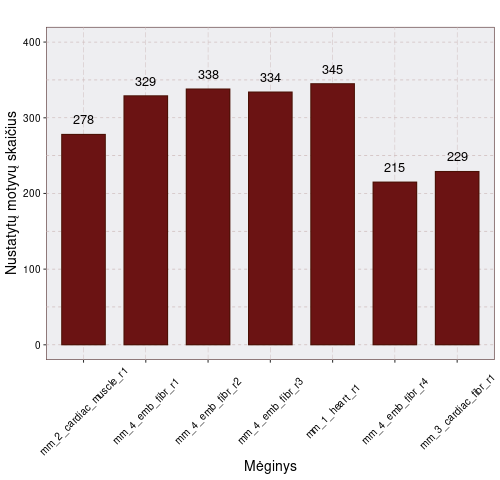
\includegraphics[width=0.6\linewidth]{../Figures/motifs_in_samples.png}
        \vspace{-2\baselineskip}
        \caption*{\small\textbf{7 pav. Identifikuotų motyvų skaičiaus
                                mėginiuose stulpelinė diagrama}}
    \end{center}
\end{figure}

Nėra neįprasta, kad paskutinių mėginių (\small\emph{emb\_fibr\_r4\_4} ir
\small\emph{crdc\_fibr\_r1\_3}) identifikuotų motyvų skaičius yra pats
mažiausias - remiantis ankstesnių analizės etapų rezultatais (4.1, 4.2, 4.3
poskyriai) šie mėginiai turi mažiausią pikų skaičių bei mažiausią juos
atitinkančių sekų rinkinį.

Nepaisant šio atitikimo, remiantis 4.1 poskyrio rezultatais mėginys
\small\emph{heart\_r1\_1} turi \(\sim\) 40 tūkst. daugiau pikų nei
\small\emph{emb\_fibr\_r4\_4}, tačiau \emph{de novo} motyvų identifikacijos
etape šiame mėginyje buvo nustatytas didžiausias motyvų skaičių (345 motyvai).
Nustatyti motyvai yra \(\sim\)12 nukleotidų ilgio.

Patikrinus, kiek vienodų motyvų aptinkama visuose mėginiuose, buvo nustatyta,
kad 131 motyvas yra būdingas visiems analizuojamiems mėginiams.

\subsection{\emph{De novo} nustatytų motyvų biologinės funkcijos}
Identifikavus motyvus, buvo nustatytos su šiais motyvais susijusių genų
funkcijos. Remiantis atliktos paieškos UniProtKB\cite{UNIPROTKB} duomenų
bazėje rezultatais, trečioje lentelėje (3 lentelė) pateikti motyvai:

\begin{enumerate}
    \item \textbf{Tbx6:} Dalyvauja ląstelių proliferacijos ir organizacijos
        procesuose, signalinių kelių valdyme, kardioblastų diferenciacijoje.
    \item \textbf{Tbet:} Dalyvauja imuninės sistemos, baltymų metabolinių
        kelių procesuose. Taip pat pasireiškia organizmui reaguojant į
        dirgiklius.
    \item \textbf{Eomes:} Dalyvauja įvairių ląstelių (pavyzdžiui,
        kardiomiocitų) diferenciacijoje, neurogenezėje, kamieninių ląstelių
        populiacijos palaikyme.
    \item \textbf{Mef2b:} Dalyvauja įvairių ląstelių diferenciacijoje.
    \item \textbf{Mef2c:} Dalyvauja ląstelių apoptozėje, kraujagyslių
        formavimęsi, pradinės embrionų širdies vystymęsi.
    \item \textbf{Mef2d:} Dalyvauja suaugusių organizmų širdies vystymęsi,
        kremzlinių bei kaulinių ląstelių diferenciacijoje.
    \item \textbf{TRPS1:} Dalyvauja kremzlinių ląstelių diferenciacijoje,
        skeleto vystymęsi, būdingas neigiamas transkripcijos reguliavimas.
    \item \textbf{GATA3:} Dalyvauja aortos vožtuvų formavimęsi, širdies
        prieširdžių morfogenezėje, embrionų organų vystymęsi, eritrocitų
        diferenciacijoje.
    \item \textbf{GATA4:} Dalyvauja širdies ląstelių diferenciacijoje,
        širdies raumens regeneracijoje, embrionų širdies formavimęsi.
    \item \textbf{Fos:} Dalyvauja atsako į jonus (kadmio, kalcio),
        citokinus bei progesteroną procesuose. Taip pat aktyvus nervų sistemos
        vystymosi metu.
    \item \textbf{Fra1:} Dalyvauja ląstelės ciklo valdyme, apoptoziniuose
        procesuose bei embrionų vystymosi gimdoje procesuose.
    \item \textbf{Fra2:} Dalyvauja teigiamoje fibroblastų proliferacijoje,
        atsako į estradiolio - moteriško lytinio hormono - procesuose.
\end{enumerate}

Apibendrinus gautus biologinių funkcijų rezultatus, identifikuoti motyvai
atlieka svarbią funkciją organizmų vystymosi bei įvairių organų formavimosi
eigoje. Ypač svarbūs transkripcijos faktoriai, kurie dalyvauja ląstelių
diferenciacijoje (pvz., kardioblastų) bei širdies dalių formavimęsi, nes šie
transkripcijos faktoriai galėtų prisidėti širdies audinių regeneracijos.

\newpage

%%%%%%%%%%%%
% IŠVADOS
%%%%%%%%%%%%

\section{Išvados}
Atlikus Tbx5 transkripcijos faktoriaus analizę su skirtingais naminės pelės
ląstelių mėginiais, kuriems buvo taikyti skirtingi poveikiai, gauti rezultatai
buvo apibendrinti:

\begin{itemize}
    \item Iš duomenų bazės atsirinkti tinkamiausi mėginiai su panašiomis
        širdies audinių ląstelėmis, tačiau skirtingais taikytais poveikiais.
    \item Nepaisant panašių ląstelių analizavimo, skirtingų modifikacijų
        pritaikymas bei galimas netikslus ChIP sekoskaitos duomenų paruošimas
        lemia akivaizdžius duomenų skirtumus.
    \item Tbx5 motyvo atitikimų skaičius tarp skirtingais poveikiais veiktų
        ląstelių mėginių skiriasi itin stipriai.
    \item De novo identifikuoti motyvai yra susiję su ląstelių diferenciacija
        bei audinių regeneracija organizmo vystymosi eigoje.
\end{itemize}

\newpage

%%%%%%%%%%%%%%%%%%%%%%%%%%
% LITERATŪROS ŠALTINIAI
%%%%%%%%%%%%%%%%%%%%%%%%%%

\bibliographystyle{plain}
\begin{thebibliography}{99}

\bibitem{REGENERATION} Kate MacCord, Jane Maienschein (2019) Philosophy of
Biology: Understanding regeneration at different scales eLife 8:e46569
https://doi.org/10.7554/eLife.46569

\bibitem{ORGANISMS} Mehta AS, Singh A. Insights into regeneration tool box:
An animal model approach. Dev Biol. 2019 Sep 15;453(2):111-129.
doi: 10.1016/j.ydbio.2019.04.006. Epub 2019 Apr 13. PMID: 30986388;
PMCID: PMC6684456.

\bibitem{GTRD} GTRD: an integrated view of transcription regulation.
Kolmykov S, Yevshin I, Kulyashov M, Sharipov R, Kondrakhin Y, Makeev VJ,
Kulakovskiy IV, Kel A, Kolpakov F Nucleic Acids Res. 2021 Jan
8;49(D1):D104-D111.

\bibitem{UCSCGB} UCSC Genome Browser: Kent WJ, Sugnet CW, Furey TS, Roskin KM,
Pringle TH, Zahler AM, Haussler D. The human genome browser at UCSC. Genome Res.
2002 Jun;12(6):996-1006.

\bibitem{ARTCL1} He A, Kong SW, Ma Q, Pu WT. Co-occupancy by multiple cardiac
transcription factors identifies transcriptional enhancers active in heart.
Proc Natl Acad Sci U S A. 2011 Apr 5;108(14):5632-7.
doi: 10.1073/pnas.1016959108. Epub 2011 Mar 17. PMID: 21415370;
PMCID: PMC3078411.

\bibitem{ARTCL2} Hashimoto H, Wang Z, Garry GA, Malladi VS, Botten GA, Ye W,
Zhou H, Osterwalder M, Dickel DE, Visel A, Liu N, Bassel-Duby R, Olson EN.
Cardiac Reprogramming Factors Synergistically Activate Genome-wide Cardiogenic
Stage-Specific Enhancers. Cell Stem Cell. 2019 Jul 3;25(1):69-86.e5.
doi: 10.1016/j.stem.2019.03.022. Epub 2019 May 9. PMID: 31080136;
PMCID: PMC6754266.

\bibitem{ARTCL3} Stone NR, Gifford CA, Thomas R, Pratt KJB, Samse-Knapp K,
Mohamed TMA, Radzinsky EM, Schricker A, Ye L, Yu P, van Bemmel JG, Ivey KN,
Pollard KS, Srivastava D. Context-Specific Transcription Factor Functions
Regulate Epigenomic and Transcriptional Dynamics during Cardiac Reprogramming.
Cell Stem Cell. 2019 Jul 3;25(1):87-102.e9. doi: 10.1016/j.stem.2019.06.012.
PMID: 31271750; PMCID: PMC6632093.

\bibitem{JCKSLAB} Jackson Laboratory (RRID:SCR\_004633).

\bibitem{R} R Core Team (2022).
R: A language and environment for statistical computing. R Foundation
for Statistical Computing, Vienna, Austria. URL https://www.R-project.org/.

\bibitem{SCIK}Scikick. Utility for executing collections of computational
notebooks.\\
URL https://petronislab.camh.ca/pub/scikick/stable/docs/report/out\_html/introduction.html

\bibitem{R_TRACK} M. Lawrence, R. Gentleman, V. Carey: "rtracklayer: an {R}
package for interfacing with genome browsers". Bioinformatics 25:1841-1842.

\bibitem{R_GGPLOT} H. Wickham. ggplot2: Elegant Graphics for Data Analysis.
Springer-Verlag New York, 2016.

\bibitem{BBTOBED} BigWig and BigBed tools: Kent WJ, Zweig AS, Barber G,
Hinrichs AS, Karolchik D. BigWig and BigBed: enabling browsing of large
distributed data sets. Bioinformatics. 2010 Sep 1;26(17):2204-7.

\bibitem{BEDTOOLS} Quinlan AR, Hall IM. BEDTools: a flexible suite of
utilities for comparing genomic features. Bioinformatics. 2010 Mar
15;26(6):841-2. doi: 10.1093/bioinformatics/btq033. Epub 2010 Jan 28.
PMID: 20110278; PMCID: PMC2832824.

\bibitem{GET_FASTA} BEDTools komandinės eilutės įrankis. Programų rinkinio
programa \emph{getfasta}.\\
Prieiga per https://bedtools.readthedocs.io/en/latest/content/tools/getfasta.html
[žiūrėta 2022-06-03].

\bibitem{BIOSTR} Pagès H, Aboyoun P, Gentleman R, DebRoy S (2022). \_Biostrings:
Efficient manipulation of biological strings\_. R package version
2.64.0, <https://bioconductor.org/packages/Biostrings>.

\bibitem{HOCOMOCO} HOCOMOCO: towards a complete collection of transcription
factor binding models for human and mouse via large-scale ChIP-Seq analysis
Ivan V. Kulakovskiy; Ilya E. Vorontsov; Ivan S. Yevshin; Ruslan N. Sharipov;
Alla D. Fedorova; Eugene I. Rumynskiy; Yulia A. Medvedeva; Arturo Magana-Mora;
Vladimir B. Bajic; Dmitry A. Papatsenko; Fedor A. Kolpakov; Vsevolod J. Makeev
Nucl. Acids Res., Database issue, gkx1106 (11 November 2017)
doi: 10.1093/nar/gkx1106

\bibitem{HOMER} Heinz S, Benner C, Spann N, Bertolino E et al. Simple
Combinations of Lineage-Determining Transcription Factors Prime cis-Regulatory
Elements Required for Macrophage and B Cell Identities. Mol Cell 2010 May
28;38(4):576-589. PMID: 20513432.

\bibitem{UPSETR} Jake R. Conway, Alexander Lex, Nils Gehlenborg. UpSetR: An R
Package For The Visualization Of Intersecting Sets And Their Properties
Bioinformatics, 33(18): 2938-2940, doi:10.1093/bioinformatics/btx364, 2017.

\bibitem{UNIPROT} The UniProt Consortium UniProt: the universal protein
knowledgebase in 2021 Nucleic Acids Res. 49:D1 (2021).

\bibitem{UNIPROTKB} Boutet E, Lieberherr D, Tognolli M, Schneider M, Bairoch A.
UniProtKB/Swiss-Prot Methods Mol. Biol. 406:89-112 (2007)

\bibitem{HEART_CELL_DIFF_ARTCL} Drowley L, Koonce C, Peel S, et al. Human
Induced Pluripotent Stem Cell-Derived Cardiac Progenitor Cells in Phenotypic
Screening: A Transforming Growth Factor-β Type 1 Receptor Kinase Inhibitor
Induces Efficient Cardiac Differentiation. Stem Cells Transl Med.
2016;5(2):164-174. doi:10.5966/sctm.2015-0114

\end{thebibliography}

\newpage

%%%%%%%%%%%%
% PRIEDAI
%%%%%%%%%%%%

\section{Priedas}

Priedų sąraše pateikiamos tarpinių rezultatų puslapio, sugeneruoto su Scikick,
bei Git repozitorijos, kurioje saugomi analizei naudoti duomenų failai,
parašyti skriptai bei pagrindinė R programa, nuorodos.

\begin{itemize}
    \item \textbf{Tarpinių rezultatų Scikick puslapis:}\\
        https://karklas.mif.vu.lt/\(\sim\)dast6577/KursinisDarbas/v1.1/peaks\_MM.html
    \item \textbf{Analizės Git repozitorija:}\\
        https://github.com/dansta0804/TF\_analysis.git
  \end{itemize}

\end{document}
